\documentclass[compress, hide notes]{beamer}

\usetheme{Madrid}
\useoutertheme[subsection=false]{smoothbars} % Beamer Outer Theme
\setbeamertemplate{blocks}[rounded][shadow=false]
\setbeamertemplate{items}[square]
\useinnertheme{rectangles} 
\setbeamertemplate{headline}
{%
	\begin{beamercolorbox}{section in head/foot}
		\vskip2pt\insertsectionnavigationhorizontal{\textwidth}{}{}\vskip2pt
	\end{beamercolorbox}
}


%fonte arial
\renewcommand{\rmdefault}{phv} % Arial
\renewcommand{\sfdefault}{phv} % Arial


\useoutertheme[subsection=false]{smoothbars} % Beamer Outer Theme
\useinnertheme{rectangles} 

\usepackage[utf8]{inputenc}
\usepackage[T1]{fontenc}
\usepackage[brazil]{babel}
\usepackage{verbatim}
\usepackage{graphicx}
\usepackage{url}
\usepackage{float}    
\usepackage[]{subfigure}
\usepackage{graphicx,color, amsmath, url}
\usepackage{scalefnt}
\usepackage{multicol}

\newcommand{\aspas}[1]{``#1''}

\graphicspath{{img/}}

	
\setbeamertemplate{navigation symbols}{}


\hyphenation{com-pu-ta-cio-nais}

\hyphenation{com-po-nen-te}

\title[Autômatos Celulares]{Teoria de Autômatos Celulares --\\ Inteligência Artificial}
\author[Natanael R., Rodolfo L. M. G..]{Natanael Ramos, Rodolfo Labiapari Mansur Guimarães}
\institute[IFMG]{Instituto Federal de Educação, Ciência e Tecnologia de Minas Gerais -\\ \textit{campus} Formiga}

\begin{document}
\frame{\titlepage}

\section{Introdução}

\subsection{Sistemas Complexos}

\begin{frame}{Sistemas Complexos}% \cite{ufmg}}
	
	\begin{itemize}
	
		\item Muitos fenômenos da natureza podem ser modelados por meio de equações obtidas pela observação destes.
		
		\bigskip
		
		\item Porém existem fenômenos difíceis de serem modelados por equações, tais como crescimento/redução de populações, o cérebro, propagações de doenças, entre outros.
			
	\end{itemize}
\end{frame}


\begin{frame}{Sistemas Complexos \cite{ufmg}}
	
	\begin{itemize}
	
		\item Tais sistemas possuem um grande número de agentes, que apesar de aparentarem independência, interagem entre si, e devido a essas interações permitem, muitas vezes, que o sistema como um todo seja auto-organizado.
		
		\bigskip
		
		\item Regras locais produzem comportamento global.
		
		\bigskip
		
		\item Regras locais dependem das relações entre os diversos agentes que compõem o sistema.
			
	\end{itemize}
\end{frame}

\subsection{História}

\begin{frame}{História \cite{ufmg}}
	
	\begin{itemize}
 		\setlength\itemsep{12pt}
	
		\item Conceituação de novas técnicas computacionais que poderiam ser utilizadas na modelagem matemática de sistemas complexos em meados de 40
        
        \item Sistemas como \cite{ufmg}:
        
        \begin{itemize}
 			\setlength\itemsep{6pt}
        	\item populações;
            \item cérebro;
            \item propagações de doenças;
           	\item entre outros.
        \end{itemize}
		
		\item John von Neumann e Stanislaw Ulam foram um dos maiores contribuidores para o desenvolvimento das tecnologias da época \cite{neumann}
			
	\end{itemize}
\end{frame}

\begin{frame}{História}

	\center
	\begin{minipage}[t]{0.45\linewidth}\centering
		
		\begin{figure}[!htb]
			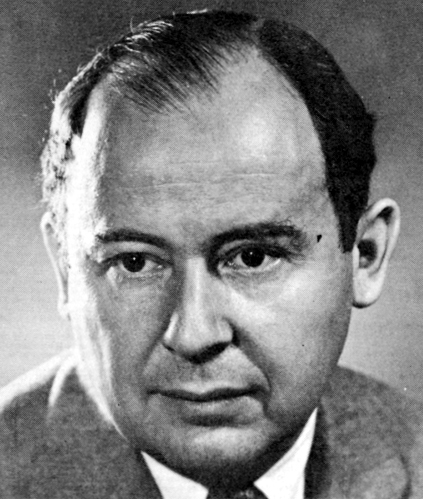
\includegraphics[width=0.77\textwidth]{img/neumann.jpg}
			\label{newmann}
			\caption{John von Neumann}
		\end{figure}
			
	\end{minipage}
	\begin{minipage}[t]{0.45\linewidth}\centering
			
		\begin{figure}[!htb]
			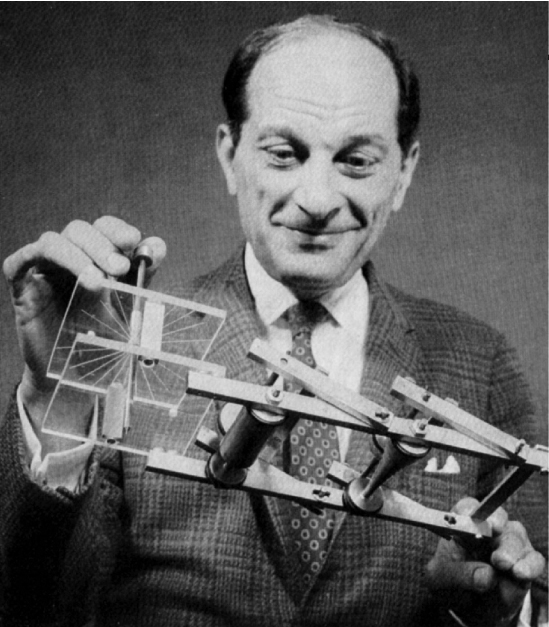
\includegraphics[width=0.8\textwidth]{img/ulam.jpg}
			\label{ulam}
			\caption{Stanislaw Ulam}
		\end{figure}
	\end{minipage}
\end{frame}

\begin{frame}{História \cite{uepg}}
	\begin{itemize}
 		\setlength\itemsep{12pt}
		\item Os objetivos eram:
        \begin{itemize}
        \setlength\itemsep{6pt}
        	\item Utilizá-los para a idealização de sistemas biológicos. Isso sobre auto-reprodução;
			\item Desenvolvimento de regras matemáticas que simulassem a natureza.
            \item Questionamento de Neumann: que tipo de organização lógica é suficiente para um autômato ser capaz de reproduzir a si próprio?
        \end{itemize}
			
		\item Tais regras seriam as mesmas para todos os componentes de um determinado sistema.
		
		\item A partir de uma configuração inicial aleatória, cada componente do sistema passaria por uma evolução influenciada por seus vizinhos e um conjunto de regras
		
	\end{itemize}
\end{frame}

\begin{frame}{História}
	\begin{itemize} 
    	\item Embora as regras sejam simples e bem conhecidas, a situação dos vizinhos pode variar indefinidamente podendo gerar novos sistemas não previstos facilmente \cite{uepg}
		%\item Embora as regras sejam as mesmas para todos os componentes, a situação dos vizinhos pode variar indefinidamente, podendo gerar novos sistemas e até chegar a sua auto-reprodução \cite{uepg}.
	
		\bigskip
    
		\item Hoje, o objetivo não é descrever um sistema complexo com equações complexas, mas deixar a complexidade surgir da iteração de indivíduos seguindo regras matemáticas simples \cite{ufmg}
        
        \bigskip
        
        \item Mostrando como um conjunto de regras básicas pode orientar um sistema complexo \cite{ufrj}
		
	\end{itemize}
\end{frame}




\section{Estrutura}
\subsection{Definição}

\begin{frame}{Definição \cite{ufmg}}
	
	\begin{itemize}
 		\setlength\itemsep{12pt}
	
		\item Um autômato celular possui:
		
		\begin{itemize}
 			\setlength\itemsep{6pt}
		
			\item Estrutura (\aspas{\textit{Lattice}}): geometria de cada célula:
            \begin{itemize}
 			\setlength\itemsep{1pt}
				\item[-] Quadrada;
                \item[-] Hexagonal;
                \item[-] Triangular.
			\end{itemize}
			
			\item Uma vizinhança;
			
			\item Uma regra de transição local. 
		
		\end{itemize}
		\pause
        \bigskip
	
		\item É definida formalmente como uma 4-tuplas $\mathbb{U = (L, Q, R}, \rho)$ onde:
		
		\begin{itemize}
 			\setlength\itemsep{6pt}
		
			\item $\mathbb{L}$: é a estrutura \aspas{\textit{lattice}}, que é  tipo de rede de contato entre os componentes do sistema;
			
			\item $\mathbb{Q}$: é o conjunto de estados;
						
			\item $\mathbb{R}$: é a vizinhança;
									
			\item $\rho$: é a regra de transição local.
		
		\end{itemize}
	\end{itemize}
\end{frame}

\begin{frame}{Definição \cite{ufmg} - ($\mathbb{U = (L, Q, R}, \rho)$)}
	\begin{itemize}
 		\setlength\itemsep{12pt}
	
		\item Uma célula arbitrária do \textit{lattice} $\mathbb{L}$ é denotada por $x,\ x \in \mathbb{L}$ onde x possui comprimento infinito ou não:
        \begin{itemize}
			\item $x_{i}$: Célula de um \textit{Lattice} de 1 dimensão (vetor);
            \item $x_{i,j}$: Célula de um \textit{Lattice} de 2 dimenstões (matriz);
            \item $x_{i,j,k}$: Célula de um \textit{Lattice} de 3 dimenstões (cubo).
		\end{itemize}
		
		\item Conjunto $\mathbb{Q}$:
        	\begin{itemize}
              \item O conjunto de estados que uma célula pode assumir;
              \item Pode assumir valores arbitrários;
              \item É composto por \textit{k} estados.
			\end{itemize}
	
    	\item Estados de uma célula:
        \begin{itemize}
          \item $x^t$ indica a geração/instante de tempo $t$ do estado daquela célula

          \item $\mathbb{R}(x)^t$, ou $(y^t_ 1, \ldots, y^t_ {vt})$ indica o estado da vizinhaça\footnote{Ou $(y^t_ 1, \ldots, y^t_ {vt})$, onde $vt$ é o comprimento da vizinhança.}
          %\item O estado da célula $x$ no instante de tempo $t$ é indicado por $x^t$ e o estado da vizinhança por $\mathbb{R}(x)^t$, ou $(y^t_ 1, \ldots, y^t_ {vt})$, onde $vt$ é o comprimento da vizinhança.
		\end{itemize}
        
		\item Alteração de um estado é dada pela função: $x^{t+1} = \rho(\mathbb{R}(x)^t)$
		
	\end{itemize}
\end{frame}


\subsection{Dimensão}
\begin{frame}{Dimensão \cite{ufmg}}
	
	\begin{itemize}
 		\setlength\itemsep{12pt}
		
		\item Os elementos constituintes do autômato celular são as células e seus estados
		\begin{itemize}		
 		\setlength\itemsep{6pt}
          \item Uma célula é o local onde é guardado um certo estado

          \item Cada célula tem apenas um único estado
		\end{itemize}
	\end{itemize}
	
	\begin{figure}[h]
		\center
		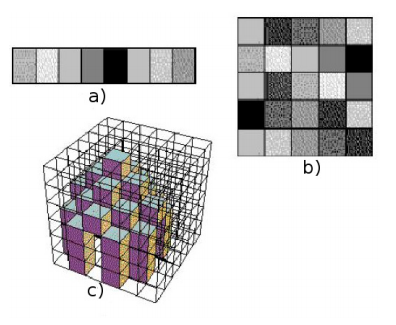
\includegraphics[width=0.4\textwidth]{dimensao.PNG}
		\caption{Dimensão: a) uma, b) duas e c) três \cite{ufmg}.}
	\end{figure}
\end{frame}
	
    
\subsection{Formato das células}
\begin{frame}{Formato das células \cite{ufmg}}
	
	\begin{itemize}
		\item Pode assumir geometrias regulares como célula quadrada, triangular e hexagonal.
	\end{itemize}
	
	\begin{figure}[h]
		\center
		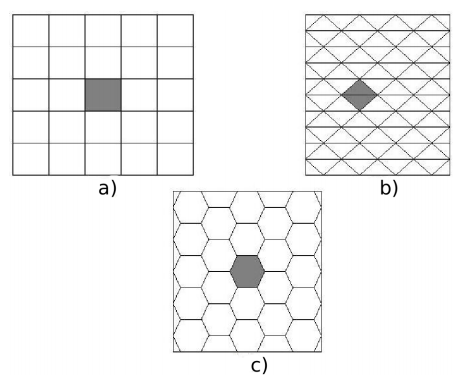
\includegraphics[width=0.5\textwidth]{formatos.PNG}
		\caption{Formatos: a) quadrada, b) triangular e c) hexagonal \cite{ufmg}.}
	\end{figure}
		
\end{frame}	


\subsection{Regras}
\begin{frame}{Vizinhanças e Regras \cite{ufmg}}
	
    \begin{itemize}
    \setlength\itemsep{14pt}
    
    	\item Para definir o novo estado da célula, deve-se definir:

        \begin{itemize}
            \setlength\itemsep{6pt}

            \item Quais células são vizinhas a uma determinada célula.

            \item Qual regra de transição será utilizada para mudança de estado de uma célula.

        \end{itemize}
        
        \item Ao final, terá o valor do próximo instante da célula, ou seja, o novo estado da célula.
        
        \item Existe vários tipos de seleção de vizinhança de uma célula:
	\end{itemize}
\end{frame}

\begin{frame}

	\begin{minipage}[t]{0.48\linewidth}\centering
		
        \begin{block}{\textbf{Vizinhança de von Neumann}}
			Considera apenas quatro células como vizinhas da célula que será atualizada.
		\end{block}
        
        \begin{figure}[h]

          \center

          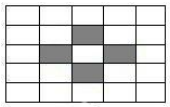
\includegraphics[width=0.7\textwidth]{vizinNewmann.PNG}
          \caption{Vizinhança de Neumann \cite{ufmg}.}

        \end{figure}

	\end{minipage}\hfill
	\begin{minipage}[t]{0.48\linewidth}\centering
 		
        \begin{block}{\textbf{Vizinhança de Moore}}
		Considera oito células como vizinhas da célula que será atualizada.
		\end{block}
        
          \begin{figure}[h]

              \center

              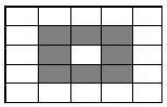
\includegraphics[width=0.7\textwidth]{vizinMoore.PNG}
              \caption{Vizinhança de Moore \cite{ufmg}.}

          \end{figure}

	\end{minipage}
    
    \bigskip
    
    \begin{itemize}
		\item Ambos com raio de vizinhança igual a 1, ou seja, apenas 1 nível de avanço na vizinhança.
	\end{itemize}
\end{frame}


\begin{frame}{Vizinhanças e Regras \cite{ufmg}}
	
	\begin{block}{\textbf{Vizinhança de Moore Estendida}} 
    	Considera um raio de vizinhança igual a dois\footnote{Duas camadas (linhas e colunas) são consideradas.}, assim a vizinhança da célula que será atualizada será igual a 25 células ao total.
	\end{block}
    
	\begin{figure}[h]
		
			\center
							
			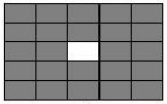
\includegraphics[width=0.5\textwidth]{vizinMooreE.PNG}
			\caption{Vizinhança de Moore Estendida \cite{ufmg}.}
			
		\end{figure}
	
\end{frame}

\begin{frame}{Vizinhanças e Regras \cite{ufmg} - Exemplo Moore}
	\begin{itemize}
        \setlength\itemsep{15pt}
		\item Exemplo de transição de estados num autômato:
        \begin{itemize}
            \setlength\itemsep{6pt}
			\item Seis estados (1 a 5 e vazio);
            \item Vizinhança de Moore (simples);
            \item ``\textit{Lattice}'' quadrado.
		\end{itemize}
		
        
		\item Algumas regras de transição do exemplo:
		
        \begin{itemize}
        \setlength\itemsep{6pt}

              \item Uma célula em estado \textbf{4}
              muda para o estado \textbf{2}
              \textit{\textbf{se}} as oito células vizinhas estejam em estado \textbf{3};

              \item Uma célula com estado \textbf{1}
              muda para o estado \textbf{5}
              se duas células vizinhas estejam em estado \textbf{3 e} o resto da vizinhança \textbf{vazio}.

          \end{itemize}
	\end{itemize}
\end{frame}
	
    
\begin{frame}{Vizinhanças e Regras}
	
	\begin{minipage}[t]{0.38\linewidth}\centering

        \begin{itemize}

              \item Uma célula em estado \textbf{4}
              muda para o estado \textbf{2}
              \textit{\textbf{se}} as oito células vizinhas estejam em estado \textbf{3};
				\bigskip
              \item Uma célula com estado \textbf{1}
              muda para o estado \textbf{5}
              se duas células vizinhas estejam em estado \textbf{3 e} o resto da vizinhança \textbf{vazio}.

          \end{itemize}

	\end{minipage}\hfill
	\begin{minipage}[t]{0.58\linewidth}\centering
        
        \begin{figure}[h]
            \center
            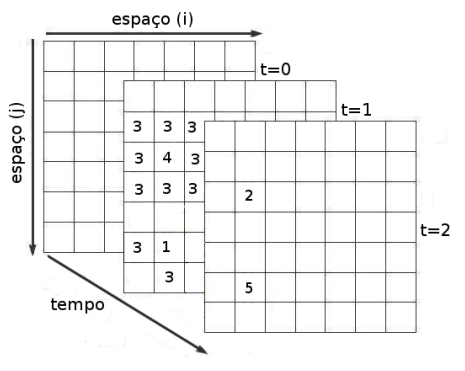
\includegraphics[width=1\textwidth]{exTransicao.PNG}
            \caption{Autômato celular com vizinhança de Moore \cite{ufmg}.}
        \end{figure}
	\end{minipage}
	
\end{frame}
	
    
\section{Autômato Celular  Unidimensional}

\subsection{Características}

\begin{frame}{Uma Dimensão \cite{pt}}
	
	\begin{itemize}
        \setlength\itemsep{11pt}
		\item São constituídos por uma grade linear de células, assim: 
        
        \begin{itemize}
        	\setlength\itemsep{6pt}
			\item Cada geração é graficamente visualizada numa grade unidimensional;
            \item A evolução das gerações em uma grade bidimensional.
		\end{itemize}
        
		\item A regra de transição $\rho(i,t)$ utiliza o estado atual de uma célula e das suas vizinhas.
		
		\item Assim o valor de $v_i$ em $i$ é dado por: $\boxed{v_i^{t+1}=\rho(v^t_{i-1}, v_i^t, v^t_{i+1})}$
		
	\end{itemize}
		\begin{figure}[h]
			\center			
			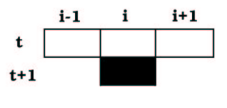
\includegraphics[width=0.32\textwidth]{uni.PNG}
			\caption{Exemplo de $\rho(i,t)$ para uma vizinhança de duas células \cite{pt}.}	
		\end{figure}
\end{frame}	

\begin{frame}{Uma Dimensão \cite{ufmg}}
	\begin{itemize}
        \setlength\itemsep{12pt}
		\item A vizinhança consiste em:
        \begin{itemize}
			\item Uma faixa $r$ de vizinhos mais próximos da célula que será atualizada na próxima geração $v_i^{t+1}$.
        \end{itemize}
		
		\item A quantidade de combinações possíveis entre os vizinhos e a própria célula, é dada por $k^{2r+1}$, onde $k$ é a quantidade de estados
		\item A quantidade de regras locais é dada por $k^{k^{2r+1}}$.
		
	\end{itemize}
	
\end{frame}	

\begin{frame}{Uma Dimensão - Efeito Borda}
	
	\begin{itemize}
        \setlength\itemsep{12pt}
		\item Problema que ocorre devido a grade linear ser constituída de um número finito de células 
        \item Se a grade possui 10 células:
        \begin{itemize}
        \setlength\itemsep{6pt}
        	\item O primeiro elemento terá como vizinhança somente o segundo;
            \item O décimo terá como vizinhança somente o nono elemento \cite{UFES}.
        \end{itemize}
	\end{itemize}
		
		\begin{figure}[h]
								
			\center
													
			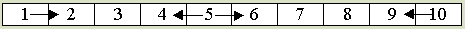
\includegraphics[width=0.7\textwidth]{borda.PNG}
			\caption{Efeito borda \cite{UFES}.}
									
		\end{figure} 
        
	\begin{block}{\textbf{Autômato elementar de uma dimensão}} 
    	É um autômato celular que possui 2 estados e raio de vizinhança igual a 1 \cite{ufmg}.
		
	\end{block}
\end{frame}

\begin{comment}

\begin{frame}{Autômatos Celulares de Uma Dimensão}
       
        \begin{figure}[h]

            \center
            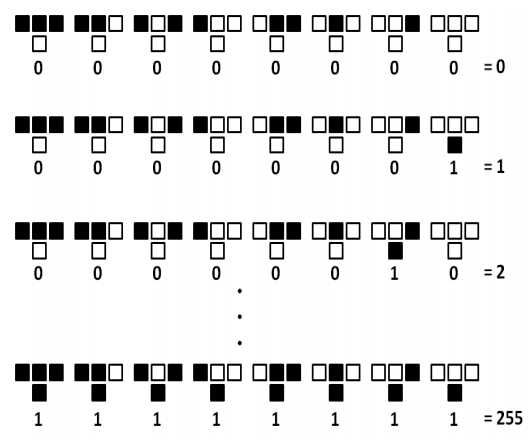
\includegraphics[width=0.5\textwidth]{255.PNG}
            \caption{Exemplo das 256 regras possíveis com $k=2$ e $r=1$ \footnote{$k$ quantidade de estados, $r$ faixas}\cite{ufmg}.}
        \end{figure}
        
\end{frame}	


\subsection{Construção}
\begin{frame}{Uma Dimensão \cite{UFES}}
	
	\begin{itemize}
	
		\item Para construir um AC unidimensional, deve-se fazer uma associação entre a regra e a vizinhança.
		
		\bigskip
		
		\item Primeiramente deve-se mudar a regra de código decimal para código binário, e alocar os dígitos binários em um vetor.
		
		\bigskip
		
		\item \textbf{Exemplo:} Regra 45
		
		\begin{table}[H]
			\centering
		    \begin{tabular}{|l|l|l|l|l|l|l|l|l|}
		    \hline
		    45     & 0 & 0 & 1 & 0 & 1 & 1 & 0 & 1 \\ \hline
		    Índice & 7 & 6 & 5 & 4 & 3 & 2 & 1 & 0 \\ \hline
		    \end{tabular}
		\end{table}
		
	\end{itemize}
	
\end{frame}

\begin{frame}{Autômatos Celulares de Uma Dimensão \cite{UFES}}
	
	\begin{itemize}
	
		\item Em seguida deve-se associar as vizinhanças, possíveis, aos seus respectivos valores do vetor da regra. Define-se para isso o valor \textbf{1} para uma célula ocupada e \textbf{0} para desocupada.
		
		\bigskip
		
		\begin{table}[H]
			\centering
		    \begin{tabular}{|l|l|l|l|l|l|l|l|l|}
		    \hline
		    Vizinhança    & 111 & 110 & 101 & 100 & 011 & 010 & 001 & 000 \\ \hline
		    Índice        & 7   & 6   & 5   & 4   & 3   & 2   & 1   & 0   \\ \hline
		    Próximo Valor & 0   & 0   & 1   & 0   & 1   & 1   & 0   & 1   \\ \hline
		    \end{tabular}
		\end{table}
		
	\end{itemize}
	
\end{frame}
\end{comment}

\begin{frame}{Uma Dimensão}
	
	\begin{figure}[h]
								
		\center
													
		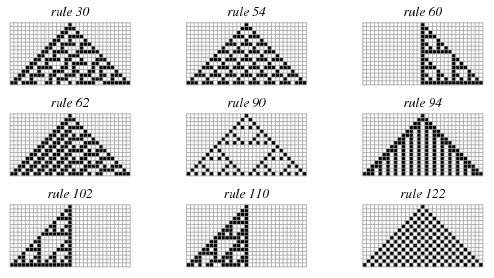
\includegraphics[width=0.9\textwidth]{rules.PNG}
		\caption{Exemplo de evolução de algumas regras de um AC elementar \cite{wolfram}.}
									
	\end{figure}
	
\end{frame}

\begin{frame}{Uma Dimensão}
	
	\begin{figure}[h]
								
		\center
													
		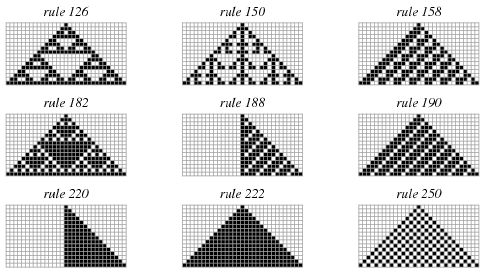
\includegraphics[width=0.9\textwidth]{rules2.PNG}
		\caption{Exemplo de evolução de algumas regras de um AC elementar \cite{wolfram}.}
									
	\end{figure}
	
\end{frame}

\subsection{Classificação de Wolfram}

\begin{frame}
	\begin{itemize}
    	\item Mais exemplos e explicação estão disponíveis em \url{http://mathworld.wolfram.com/ElementaryCellularAutomaton.html}
        \bigskip
        
        \bigskip
	
		\item Existem quatro classes básicas de comportamento para autômatos celulares unidimensionais:
        \begin{enumerate}
        	\setlength\itemsep{8pt}
			\item Classe I;
            \item Classe II;
            \item Classe III;
            \item Classe IV.
		\end{enumerate}
	\end{itemize}
\end{frame}

\begin{frame}{Comportamento \cite{ufmg}}
	
	\begin{itemize}
        
		\item \textbf{Classe I:} comportamento fixo, a evolução leva a um estado homogêneo, ou seja, todas as células no mesmo estado.	
	
		\begin{figure}[h]
											
			\center
																
			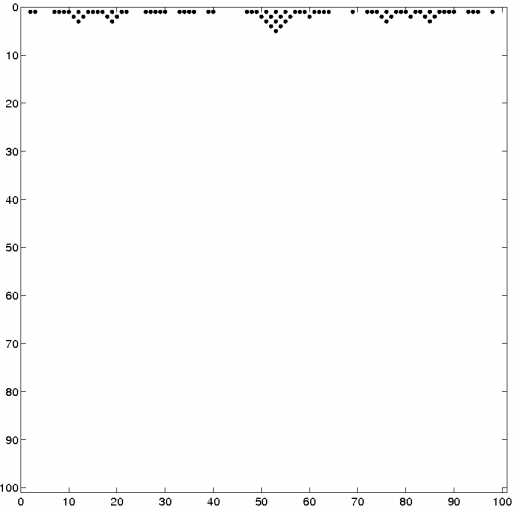
\includegraphics[width=0.48\textwidth]{32.PNG}
			\caption{Exemplo de representante da classe I, Regra 32 \cite{ufmg}.}
												
		\end{figure}
		
	\end{itemize}
	
\end{frame}

\begin{frame}{Comportamento \cite{ufmg}}
	
	\begin{itemize}
		
		\item \textbf{Classe II:} comportamento cíclico ou periódico, os autômatos geralmente criam imagens que se repetem periodicamente, com poucos períodos ou imagens estáveis.
	
		\begin{figure}[h]
											
			\center
																
			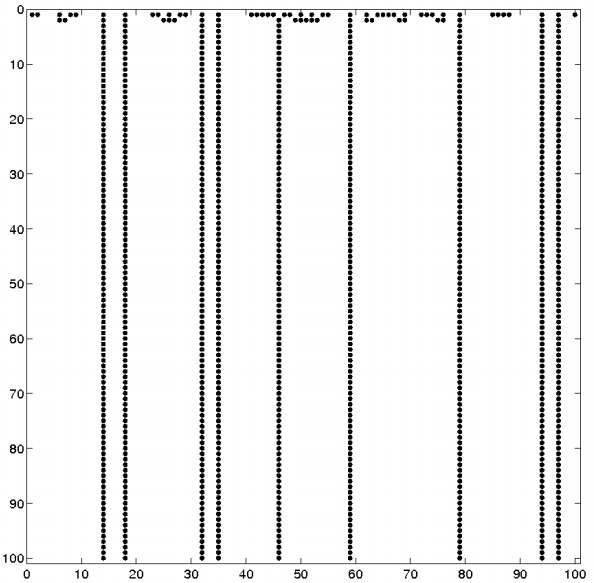
\includegraphics[width=0.45\textwidth]{36.PNG}
			\caption{Exemplo de representante da classe II, Regra 36 \cite{ufmg}.}
												
		\end{figure}
		
	\end{itemize}
	
\end{frame}

\begin{frame}{Comportamento \cite{ufmg}}
	
	\begin{itemize}
		
		\item \textbf{Classe III:} comportamento caótico, refere-se ao comportamento espaço-tempo aparentemente imprevisível. São fortemente dependentes do estado inicial.
	
		\begin{figure}[h]
											
			\center
																
			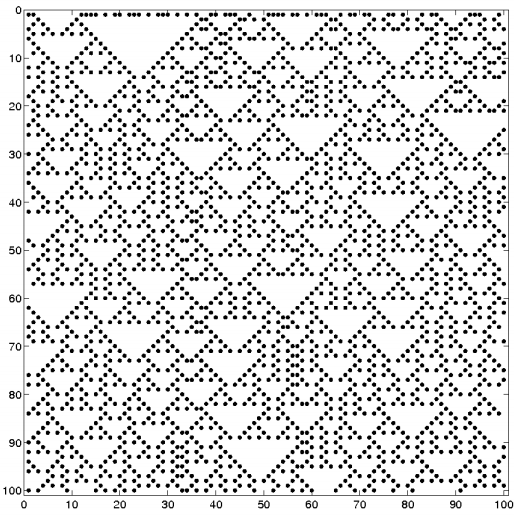
\includegraphics[width=0.42\textwidth]{18.PNG}
			\caption{Exemplo de representante da classe III, Regra 18 \cite{ufmg}.}
												
		\end{figure}
		
	\end{itemize}
	
\end{frame}

\begin{frame}{Comportamento \cite{ufmg}}
	
	\begin{itemize}
		
		\item \textbf{Classe IV:} comportamento complexo, os autômatos aparentam repetição irregular, no tempo, de padrões, a diferentes escalas e posições no espaço. Situa-se entre as classes II e III. ACs podem crescer ou contrair com o tempo.
	
		\begin{figure}[h]
											
			\center
																
			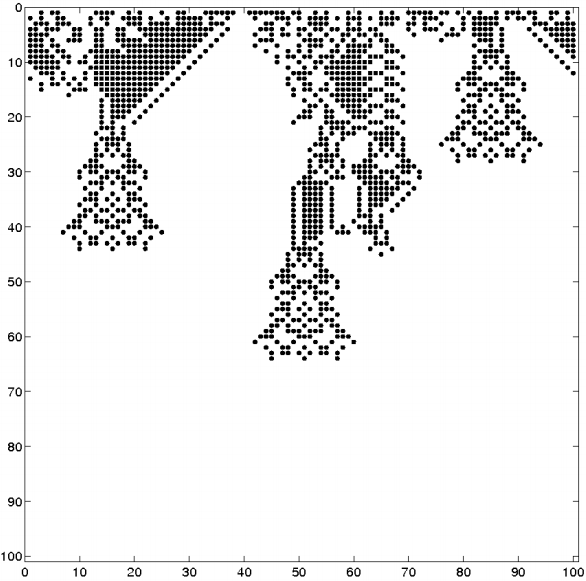
\includegraphics[width=0.4\textwidth]{20.PNG}
			\caption{Exemplo de representante da classe IV, Regra 20 \cite{ufmg}.}
												
		\end{figure}
		
	\end{itemize}
	
\end{frame}

\subsection{Utilização}

\begin{frame}{Natureza \cite{ufmg}}
	
	\begin{itemize}
		
		\item Conus \textit{textile} e autômato celular Regra 30.
		
			\begin{minipage}[t]{0.45\linewidth}\centering
				
				\begin{figure}[!htb]
			
					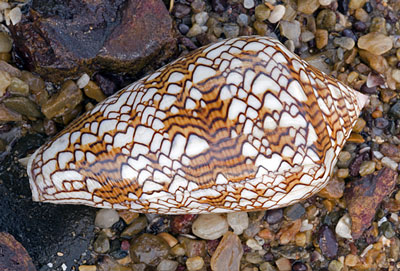
\includegraphics[width=1.0\textwidth, angle=180]{conusReal.JPG}
					\label{conusReal}
					\caption{Conus \textit{textile.}}
				
				\end{figure}
					
				\end{minipage}\hfill
			\begin{minipage}[t]{0.45\linewidth}\centering
					
				\begin{figure}[!htb]
			
					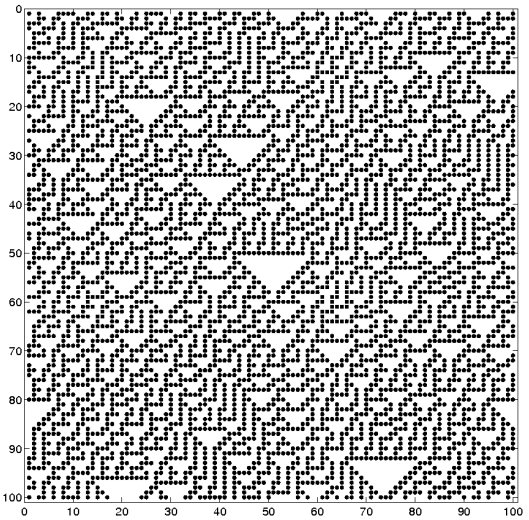
\includegraphics[width=1.0\textwidth]{30.PNG}
					\label{regra30}
					\caption{AC regra 30 \cite{ufmg}.}
				
				\end{figure}
					
			\end{minipage}
		
	\end{itemize}
	
\end{frame}

\section{AC Bidimensional}

\subsection{Características}

\begin{frame}[allowframebreaks]{Autômatos Celulares de Duas Dimensões \cite{pt}}
	
	\begin{itemize}
	
		\item São constituídos por uma matriz de células, onde cada célula (i,j) toma um valor $v_{ij}$ e é atualizado no decorrer do tempo $t$ de acordo com uma regra $\rho(i,t)$.
		
		\bigskip
		
		\item O valor de $v_i$ de uma célula $i$ é dado por: $v_{ij}^{t+1}=\rho(v_{ij}^t, v_{ij-1}^t, v_{i-1j}^t, v_{i+1j}^t, v_{ij+1}^t)$
        
        \bigskip
        
        \item Permitem várias estruturas de vizinhança e \textit{Lattice}, devido as possibilidades de combinações.
        
        \bigskip
        
        \framebreak
			
		\begin{figure}[h]
								
			\center
													
			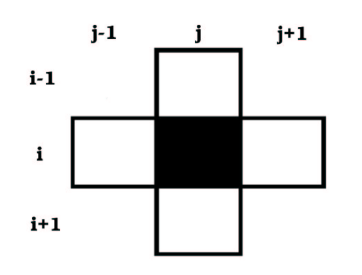
\includegraphics[width=0.4\textwidth]{bi.PNG}
			\caption{Exemplo de $\rho(i,t)$ para uma vizinhança de quatro células \cite{pt}.}
							
		\end{figure}
		
	\end{itemize}
	
\end{frame}	

\begin{frame}{Utilização \cite{ufmg}}
	
	\begin{itemize}
	
		\item Utilizado para comparações com resultados experimentais na formação de padrões em sistemas físicos.
		
		\bigskip
		
		\item Aplicações imediatas: crescimento de cristais dendríticos\footnote{É um cristal que se desenvolve como um típica árvore multi-ramificada. Um exemplo é a formação de flocos de neves.}, sistemas de reação-difusão e padrões de fluidos turbulentos.
		
	\end{itemize}
	
\end{frame}

\begin{frame}{Utilização}
	
	\begin{itemize}
	
		\item \textbf{Propagação de incêndios florestais \cite{ufmg}:}
		
		\begin{itemize}
		
			\item Se uma célula está cinza e uma das suas vizinhas está no estado branco, existe uma probabilidade não nula de no instante seguinte a célula mudar para o estado preto.
			
			\bigskip
			
			\item Se existir vento em uma certa direção a probabilidade de transição cinza para branco é maior nesta direção.

			\bigskip
			
			\item Se uma célula está no estado preto, então se manterá nesse estado indefinidamente.
			
			\bigskip
			
			\item Quando uma árvore está no estado branco ela vai se manter neste estado por duas gerações e depois ficará preta.
			
			\bigskip
			
			\item Considerou-se 4 vizinhos.
		
		\end{itemize}
		
	\end{itemize}
	
\end{frame}

\begin{frame}{Utilização}
	
	\begin{figure}[h]
								
		\center
													
		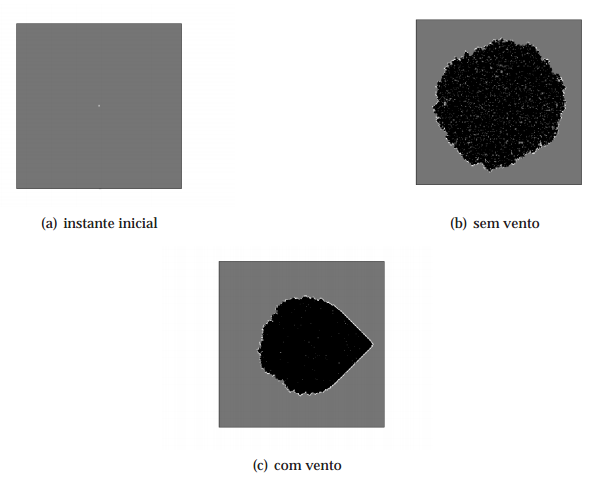
\includegraphics[width=0.7\textwidth]{incendio.PNG}
		\caption{Propagação de incêndio com vento e sem vento \cite{ufmg}.}
							
	\end{figure}
	
\end{frame}

\begin{frame}{Utilização}
	
	\begin{itemize}
	
		\item \textbf{Jogo da Vida \cite{ufmg}:}
		
		\begin{itemize}
		
			\item Desenvolvido pelo matemático John Horton Conway em 1970.
			
			\bigskip
			
			\item É um autômato celular que simula processos de evolução de células biológicas, que possui dois estados (morto e vivo) e oito vizinhos.
		
		\end{itemize}
		
	\end{itemize}
	
\end{frame}

\begin{frame}{Utilização}
	
	\begin{itemize}
	
		\item \textbf{Regras \cite{ufmg}:}
		
		\begin{itemize}
			
			\item Uma célula viva com um vizinho vivo ou nenhum vivo, morre por solidão.
			
			\bigskip
			
			\item Uma célula viva com mais do que três vizinhos vivos, morre por superpopulação.
			
			\bigskip
			
			\item Uma célula viva com 2 ou 3 vizinhos vivos, sobrevive na próximo instante.
			
			\bigskip
			
			\item Uma célula morta com exatamente 3 vizinhos vivos, nasce.
		
		\end{itemize}
		
	\end{itemize}
	
\end{frame}

\begin{frame}{Utilização}
	
	\begin{itemize}
	
		\item Pode-se notar grupos de células chamadas \aspas{piscantes} ao longo da evolução do Jogo da Vida. \textbf{Cor cinza: célula morta, Cor branca: célula viva}.
		
		\bigskip
		
		\item Tais células são blocos que alteram constantemente entre dois estados de acordo com as regras , que se forem intocadas irão piscar para sempre, isso é chamado comportamento oscilatório.
		
		\begin{figure}[h]
										
			\center
															
			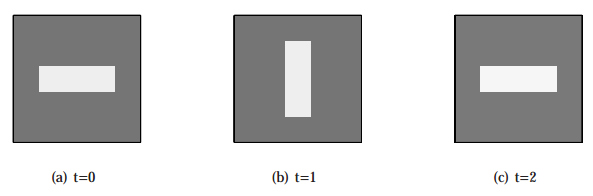
\includegraphics[width=0.7\textwidth]{piscante.PNG}
			\caption{Comportamento oscilatório \cite{ufmg}.}
									
		\end{figure}
		
	\end{itemize}
	
\end{frame}

\begin{frame}{Utilização}
	
	\begin{itemize}
	
		\item Outra estrutura encontrada são os \textit{gliders}, que deslizam em diagonal pelo AC e continuam fazendo isso até encostarem em uma célula viva.
				
		\begin{figure}[h]
										
			\center
															
			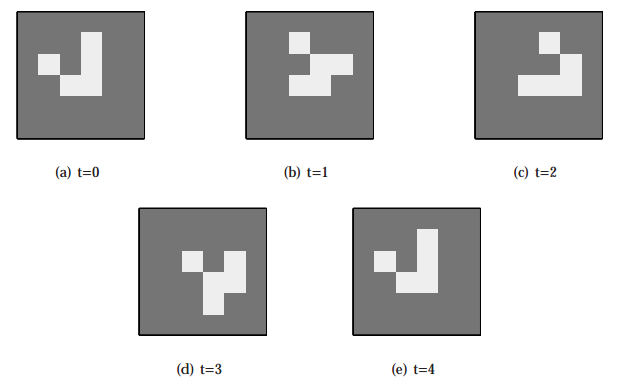
\includegraphics[width=0.7\textwidth]{glider.PNG}
			\caption{Estrutura \textit{glider} \cite{ufmg}.}
									
		\end{figure}
		
	\end{itemize}
	
\end{frame}

\begin{frame}{Utilização}
	
	\begin{itemize}
	
		\item Um outro estado que pode surgir após evoluções do Jogo da Vida é a extinção, onde todas as células morrem.
				
		\begin{figure}[h]
										
			\center
															
			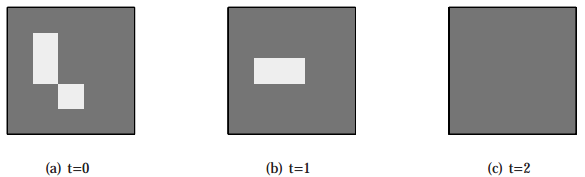
\includegraphics[width=0.7\textwidth]{extincao.PNG}
			\caption{Comportamento de extinção \cite{ufmg}.}
									
		\end{figure}
		
	\end{itemize}
	
\end{frame}

\begin{frame}{Utilização}
	
	\begin{itemize}
	
		\item É possível também observar o comportamento estável, que é quando a evolução do sistema converge para um estado permanente.
				
		\begin{figure}[h]
										
			\center
															
			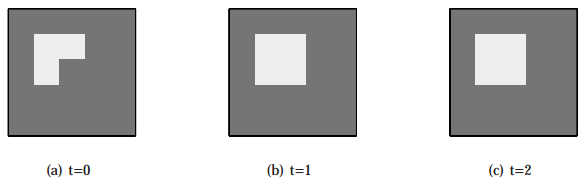
\includegraphics[width=0.7\textwidth]{estavel.PNG}
			\caption{Comportamento estável \cite{ufmg}.}
									
		\end{figure}
		
	\end{itemize}
	
\end{frame}

\begin{frame}{Utilização}
	
	\begin{itemize}
	
		\item Evolução de uma população inicial aleatória, com uma matriz de 200 x 200 células e \aspas{\textit{lattice}} quadrado.
	
	\end{itemize}
	
\end{frame}

\begin{frame}{Utilização}
		
	\begin{figure}[h]
										
		\center
															
		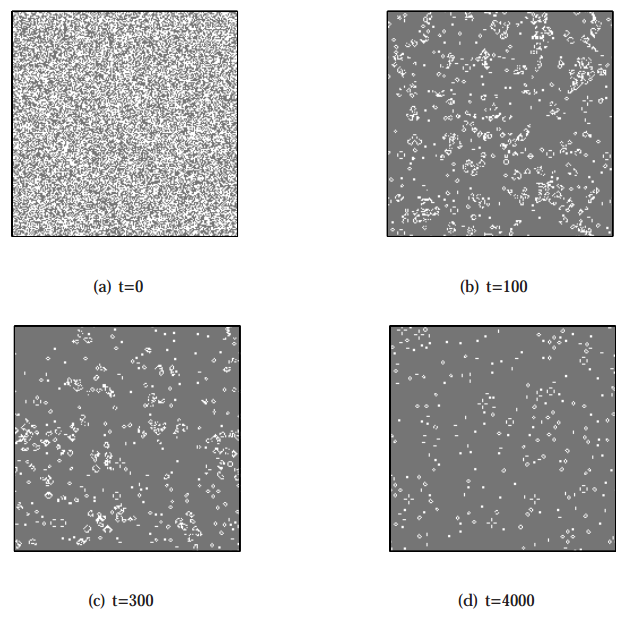
\includegraphics[width=0.6\textwidth]{gameEx.PNG}
		\caption{Evolução de uma população no Jogo da Vida \cite{ufmg}.}
									
	\end{figure}
	
\end{frame}

\section{Outras Utilizações}

\begin{frame}{Outras Utilizações \cite{pt}}
		
	\begin{itemize}
	
		\item \textbf{Formação de cristais:} como é que uma molécula de água \aspas{sabe} onde se colocar para formar um floco de neve?
	
		\begin{figure}[h]
												
			\center
																	
			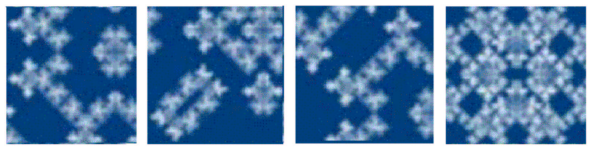
\includegraphics[width=0.8\textwidth]{cristais.PNG}
			\caption{Formação de Cristais.}
											
		\end{figure}
		
		\item Conjunto de equações diferenciais também resolveria o problema, mas o simples modelo pelo AC preserva a essência do processo de criação dessa estrutura.
        
        \item uma regra fixa que determina se o local deve ficar ocupado por uma molécula de água ou livre. 

        \item Descrição do modelo:
        
        \begin{itemize}
          \item Um vector uniforme bidimensional de células, com um conjunto pequeno de possíveis estados que dependem de um conjunto pequeno de
          células vizinhas. 
          \item A molécula de água é agregada se à sua volta estiverem pelo menos três moléculas de água a e se a  respectiva célula estiver desocupada.
        \end{itemize}
        
	\end{itemize}
	
\end{frame}

\begin{frame}{Outras Utilizações \cite{pt}}
		
	\begin{itemize}
	
		\item \textbf{Modelo de Crescimento Urbano:} é possível conjecturar como será uma cidade no futuro caso continue a seguir as mesmas políticas de ordenamento;
	
		\begin{figure}[h]
												
			\center
					
			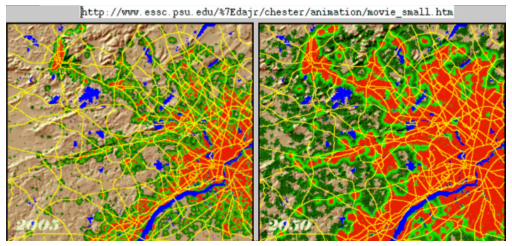
\includegraphics[width=0.8\textwidth]{cidade.PNG}
			\caption{Modelagem de uma cidade da Pensilvânia.}
											
		\end{figure}
        
        \item O desenvolvimento de uma área é baseado nos atributos das áreas a suas volta.
	
	\end{itemize}
	
\end{frame}

\begin{frame}{Outras Utilizações \cite{pt}}
		
	\begin{itemize}
	
		\item \textbf{Evolução de Epidemias:} A expansão de epidemias pode ser simulada através de autômatos celulares em que a cada célula do autômato corresponde uma área da região geográfica a analisar.
	
		\begin{figure}[h]
												
			\center
																	
			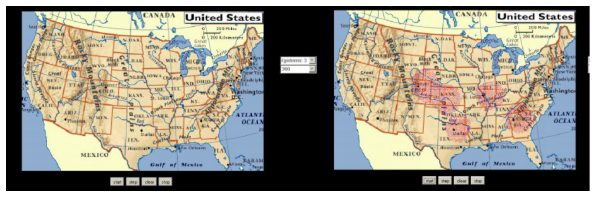
\includegraphics[width=0.8\textwidth]{epidemia.PNG}
			\caption{AC para simulação da evolução de uma epidemia.}
											
		\end{figure}
		
		\item A	infecção parte de uma célula do autômato e propaga-se segundo determinadas regras que consideram proximidade a cursos de água, vias existentes, plantações, e etc.
	
	\end{itemize}
	
\end{frame}

\begin{frame}{Outras Utilizações \cite{pt}}
		
	\begin{itemize}
	
		\item Simulação de Padrões de Crime;
		
		\bigskip
		
		\item Criptografia;
		
		\bigskip
		
		\item Colônias e Super-organismos;
		
		\bigskip
		
		\item Ecossistemas;
		
		\bigskip
		
		\item Reações Químicas.
	
	\end{itemize}
	
\end{frame}

	\begin{thebibliography}{100}
	
    	\bibitem{ufrj} LIMA, L. Z.; OLIVEIRA, P. P. M. \textbf{Jogo Da Vida}: Conceitos e Aplicações, Universidade Federal do Estado do Rio de Janeiro, 2014. Monografia. [acesso em 2015-07-20].
    
    	\bibitem{uepg} MARTINS, Caroline Collaço. \textbf{Automato Celular Aplicado no Crescimento de Câncer}. Ponta Grossa: Unidade Estadual de Ponta Grossa, 2010. Dissertação para obtenção do grau de Mestre em Ciências. [acesso 2014-08-23]. Disponível em: \url{http://fisica.uepg.br/ppgfisica/Public/Projetos/1316461681.pdf}.
    
		\bibitem{ufmg} MELOTTI, Gledson. \textbf{Aplicação de Autômatos Celulares em
		Sistemas Complexos}: Um Estudo de Caso em Espalhamento de Epidemias. Belo Horizonte: Laboratório de Modelagem, Análise e Controle de Sistemas Não-Lineares, Universidade Federal de Minas Gerais, 2009. Dissertação para obtenção do grau de Mestre em Engenharia Elétrica. [acesso 2014-08-23]. Disponível em: \url{http://www.cpdee.ufmg.br/documentos/Defesas/802/Dissertacao_Gledson_final.pdf}.

		\bibitem{pt} SOUSA, Sónia Alexandra F. S. \textbf{Autômatos Celulares}. Cidade do Porto: Departamento de Ciência de Computadores	Faculdade de Ciências da Universidade do Porto, 2001/2002. Monografia. [acesso 2014-08-23]. Disponível em: \url{http://www.di.ubi.pt/~cbarrico/Disciplinas/VidaArtificial/Download/AutomatosCelulares.PDF}.
		
		\bibitem{UFES} UFES. F\textbf{ractais e Autômatos Celulares}. Acessado em 23/08/2014. Disponível em \url{http://www.modelab.ufes.br/automato/index.htm}
	
    	\bibitem{neumann} VON NEUMANN, John et al. Theory of self-reproducing automata. IEEE Transactions on Neural Networks, v. 5, n. 1, p. 3-14, 1966.
        
        \bibitem{wolfram} WOLFRAM. \textbf{Elementary Cellular Automaton}. Acessado em 23/08/2014. Disponível em \url{http://mathworld.wolfram.com/ElementaryCellularAutomaton.html}
	
	\end{thebibliography}


\end{document}
